\documentclass{beamer}
 
\usepackage[utf8]{inputenc}
\usepackage{etoolbox}
\setbeamercovered{transparent}

% \usepackage{bm}
\usepackage{mathtools}          %loads amsmath as well
\usepackage{lmodern}
\usepackage{flexisym}
\usepackage[absolute,overlay]{textpos}

\usepackage{tikz}
\usetikzlibrary{positioning}
\usetikzlibrary{arrows}
\usetikzlibrary{shapes}
\usetikzlibrary{decorations.pathreplacing}

\tikzset{basic/.style={draw,fill=blue!20,text width=1em,text badly centered}}
\tikzset{input/.style={basic,circle}}
\tikzset{weights/.style={basic,rectangle}}
\tikzset{functions/.style={basic,circle,fill=blue!10}}
\tikzset{
  treenode/.style = {shape=rectangle, rounded corners,
                     draw, align=center,
                     top color=white, bottom color=blue!20},
  root/.style     = {treenode, font=\Large, bottom color=green!30},
  env/.style      = {treenode, font=\ttfamily\normalsize},
  dummy/.style    = {circle,draw}
  invisible/.style={opacity=0},
  visible on/.style={alt={#1{}{invisible}}},
  alt/.code args={<#1>#2#3}{%
      \alt<#1>{\pgfkeysalso{#2}}{\pgfkeysalso{#3}} % \pgfkeysalso doesn't change the path
  },
}

% \usetheme{Copenhagen}
\usetheme{EastLansing}
\usecolortheme{dolphin}
 
 
%Information to be included in the title page:

\titlegraphic{%
    \vspace*{10mm}
    \makebox[0.9\paperwidth]{%
        \raggedleft
\includegraphics[height=1.1cm,keepaspectratio]{pics/oeaw-logo.jpg}%
        \hfill%
        % \hspace*{-10mm}
        \raggedright
\includegraphics[height=1.1cm,keepaspectratio]{pics/smi-logo.jpg}%
        % \hspace*{3mm}
    }%
}

\title[Introduction to Machine learning] %optional
{Machine learning methods applied to the analysis of central exclusive production events in ALICE}
 
% \subtitle{A short story}
  
\author[Ratzenböck] % (optional, for multiple authors)
{Sebastian Ratzenböck\inst{1}}

\institute[SMI] % (optional)
{
\inst{1}%
Stefan Meyer Institut\\
Österreichische Akademie der Wissenschaften
}
  
\date[26.April 2018] % (optional)
{26. April 2018}
 
\begin{document}

%------------------------------------------------ 
\frame{\titlepage}

%------------------------------------------------ 

\begin{frame}
    \frametitle{Outline}
    \tableofcontents
\end{frame}

%------------------------------------------------ 
\section{ML: an overview} %

\begin{frame}
    \frametitle{ML: an overview}
    In general ML represents a contrast to a \emph{rule based systems}
    \begin{block}{Rule-based system}
        System that uses rules to make deductions or choices
        \begin{itemize}
            \item<1-> Domain-specific expert system
            \item<2-> Knowledge base: facts \& rules (if $\to$ then statement)
            \item<3-> Rules manually specified (by expert) $\to$ expensive, incomplete
        \end{itemize}
    \end{block}
\end{frame}

%------------------------------------------------ 

% \begin{frame}
%     \frametitle{ML: an overview}
%     In general ML represents a contrast to a \emph{rule based systems}
%     \begin{block}{Machine learning}
%         \begin{itemize}
%             \item<1-> Alorithms that learn from \emph{data} \& make predictions on \emph{data}
%             \item<2-> Automatic methods (no human needed)
%             \item<3-> Human work required for defining problem \& assessing the data
%         \end{itemize}
%     \end{block}
% \end{frame}

%------------------------------------------------ 

\begin{frame}
    \frametitle{ML: an overview}
    In general ML represents a contrast to a \emph{rule based systems}
    \begin{block}{Machine learning}
        \begin{itemize}
            \item<1-> Alorithms that learn from \emph{data} \& make predictions on \emph{data}
            \item<2-> Automatic methods $\to$ no human needed
            \item<3-> Human work required for defining problem \& assessing the data
        \end{itemize}
    \end{block}
\end{frame}

%------------------------------------------------ 

\begin{frame}
    \frametitle{Types of ML}
    \begin{columns}[T] % align columns
        \begin{column}{.48\textwidth}
            % \color{red}\rule{\linewidth}{4pt}

            \begin{itemize}
                \item <1->Supervised 
                \begin{itemize}
                    \item Classification
                    \item Regression
                \end{itemize}
                \item<2-> Unsupervised
            \end{itemize}
        \end{column}%
        \hfill%
        \begin{column}{.48\textwidth}
            \includegraphics<1>[height=4.5cm,keepaspectratio]{pics/supervised.png}%
            \includegraphics<2>[height=4.5cm,keepaspectratio]{pics/UNsupervised.png}%
            % \includegraphics<1>[height=3.5cm,keepaspectratio]{pics/supervised.png}\\%
            % \includegraphics<2>[height=3.5cm,keepaspectratio]{pics/UNsupervised.png}%
        \end{column}%
    \end{columns}
\end{frame}

%------------------------------------------------ 

\section{Rectangular cuts} %
\begin{frame}
    \frametitle{Rectangular cuts}
    \begin{columns}[T] % align columns        
        \begin{column}{.48\textwidth}
            % \color{red}\rule{\linewidth}{4pt}
            \vspace*{-10mm}
            Standard cut in one variable
            \begin{itemize}
                \item<1-> Cuts only in lower-dimensional subspaces
                \item<2-> Ignores possible dependencies between the input variables
                \item<3-> Signal might behave like BG in several observables\\ $\to$ misclassification
            \end{itemize}
        \end{column}%
        \hfill%
        \begin{column}{.48\textwidth}
            % \color{blue}\rule{\linewidth}{4pt}
            \vspace*{-10mm}
            % \hspace*{-10mm}
            \raggedright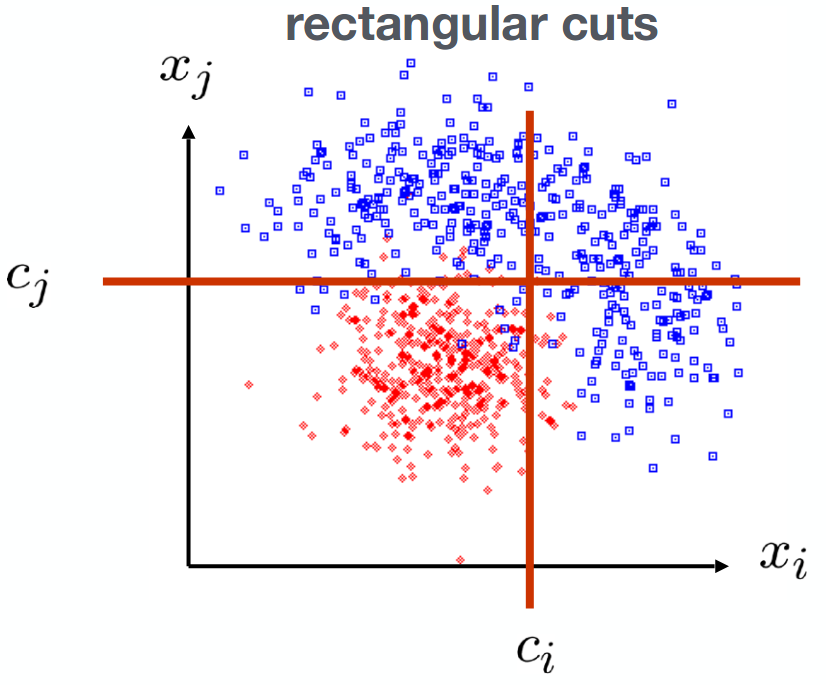
\includegraphics[height=4.3cm,keepaspectratio]{pics/mva_cuts_rectangular.png}%
            
        \end{column}%
    \end{columns}

\end{frame}

%------------------------------------------------ 

\subsection{Decision Trees}
\begin{frame}
    \frametitle{Rectangular cuts with \emph{decision trees}}
    \vspace*{-7mm}
    \begin{itemize}
        % \item Simple \& rather old model (\emph{60s, 70s})
        \item Tree-like graph $\to$ flowchart
        \item Easy to understand
        \item Either be manually modelled by experts or learned from training data
    \end{itemize}
\end{frame}

%------------------------------------------------ 

\begin{frame}
    \frametitle{Rectangular cuts with \emph{decision trees}}
    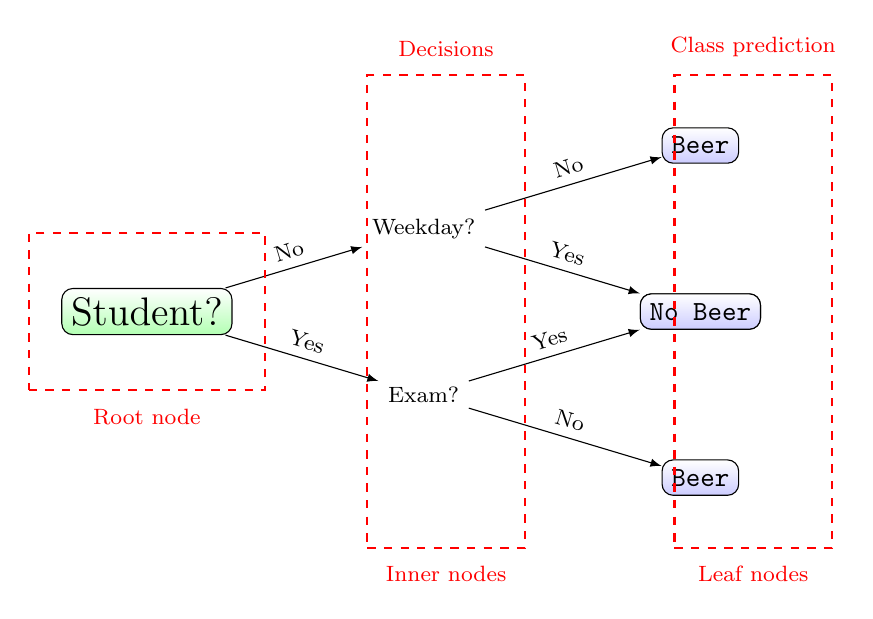
\begin{tikzpicture}
        [
            grow                    = right,
            sibling distance        = 6em,
            level distance          = 10em,
            edge from parent/.style = {draw, -latex},
            every node/.style       = {font=\footnotesize},
            sloped
        ]
	\node [root] {Student?}
        child { node [dummy] {Exam?}
                child { node [env] {Beer}
                        edge from parent node [above] {No} }
                child { node [env] {No Beer}
                        edge from parent node [above] {Yes} }                
                edge from parent node [above] {Yes} }
        child { node [dummy] {Weekday?}
                child { node [env] {No Beer}
                        edge from parent node [above] {Yes} }
                child { node [env] {Beer}
                        edge from parent node [above] {No} }                
                edge from parent node [above] {No} };
    \pause
    \node (rectroot) at (0,0) [rectangle, dashed, color=red, minimum height=2cm,minimum width=3cm,draw, thick] {};
    \node (rootbottom) [below=1mm of rectroot, color=red]  {Root node};
    \pause
    \node (rectinner) at (3.8,0) [rectangle, dashed, color=red, minimum height=6cm,minimum width=2cm,draw, thick] {};
    \node (innerbottom) [below=1mm of rectinner, color=red]  {Inner nodes};
    \node (innertop) [above=1mm of rectinner, color=red]  {Decisions};
    \pause
    \node (rectleaf) at (7.7,0) [rectangle, dashed, color=red, minimum height=6cm,minimum width=2cm,draw, thick] {};
    \node (leafbottom) [below=1mm of rectleaf, color=red]  {Leaf nodes};
    \node (leaftop) [above=1mm of rectleaf, color=red]  {Class prediction};

    \end{tikzpicture}
\end{frame}

%------------------------------------------------ 

\begin{frame}
    \frametitle{Decision tree learning}
    \vspace*{-7mm}
    \begin{block}{Training}
        \emph{Recursively} split feature space into sub-spaces at each step\\
        $\to$ Measures to evaluate split
        \begin{itemize}
            \item Error rate
            \item Information gain
            \item Gini index
        \end{itemize}
    \end{block}
\end{frame}

%------------------------------------------------ 

\subsection{Example}
\begin{frame}
    \frametitle{Decision tree learning}
    \centering\begin{tikzpicture}
        \node[inner sep=0pt] (featspace) at (0,0)
            {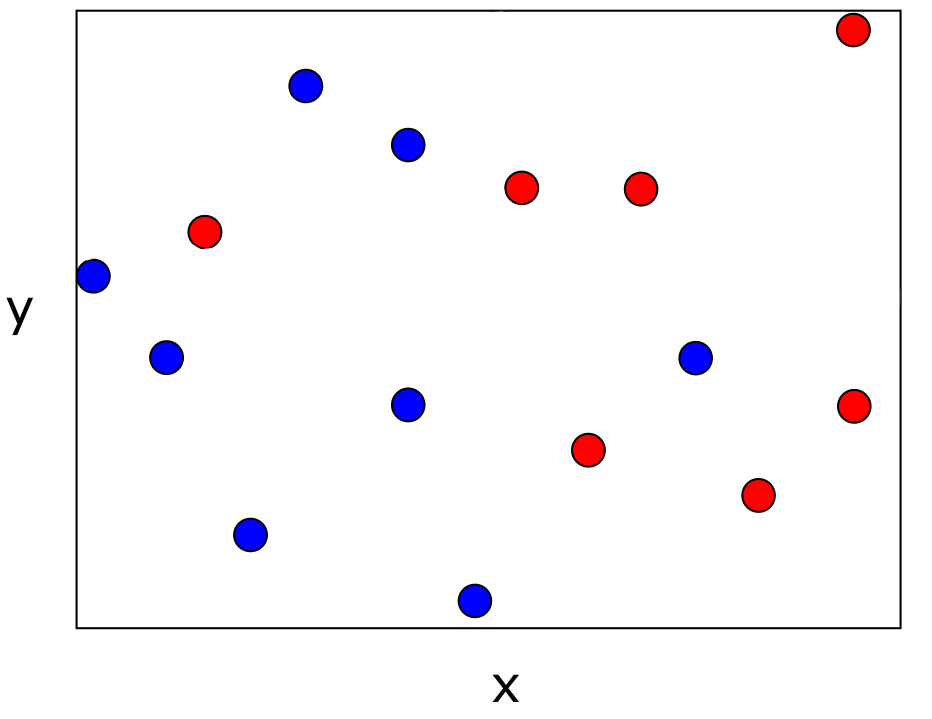
\includegraphics[height=3cm,keepaspectratio]{pics/DT-feature-space.png}};
        \node (featspaceTop) [above=1mm of featspace, color=black]  {Feature space};
        \node[inner sep=0pt] (nodes) at (3,-3.5)
            {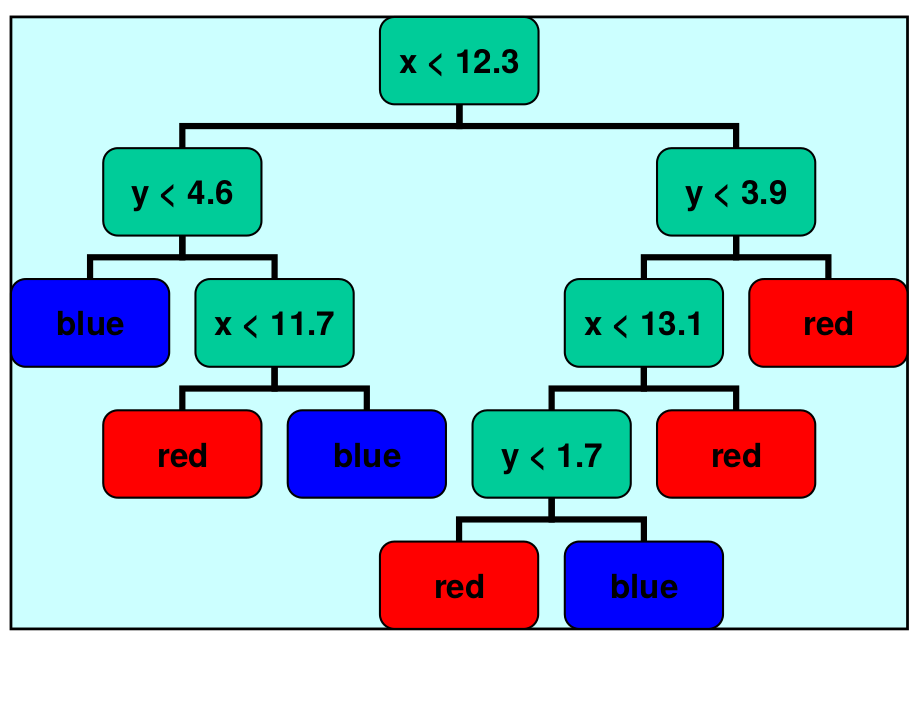
\includegraphics[height=3.3cm,keepaspectratio]{pics/DT-fullygrown_nodes.png}};%
        \node (nodesTxt) [above=1mm of nodes, color=black]  {Decision tree};
        \node[inner sep=0pt] (DTapply) at (-3,-3.5)
            {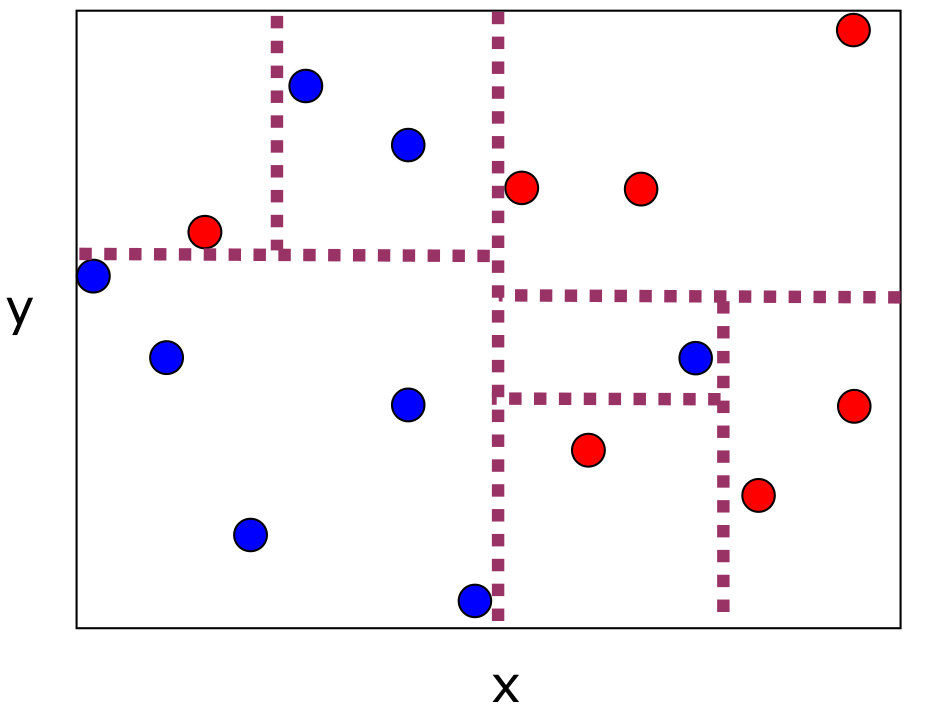
\includegraphics[height=3.3cm,keepaspectratio]{pics/DT-fullygrown_feature_space.png}};
        \node (DTTxt) [above=1mm of DTapply, color=black]  {Classification};

        \draw[->,thick] (featspace.east) to [out=0,in=90] (nodesTxt.north) node[midway,above] {};
        \draw[->,thick] (featspace.west) to [out=180,in=90] (DTTxt.north) node[midway,above] {};
    \end{tikzpicture}
\end{frame}

%------------------------------------------------ 

\begin{frame}
    \frametitle{Decision tree learning}
    1) We compute a measure for \emph{each possible split} in each feature\\\hspace*{5mm}$\to$ here \textbf{absolute error rate} (AER)
    \\
    \vspace*{3mm}
    \centering\begin{tikzpicture}
        \node[inner sep=0pt, visible on=<1>] (feat1) at (0,0)
            {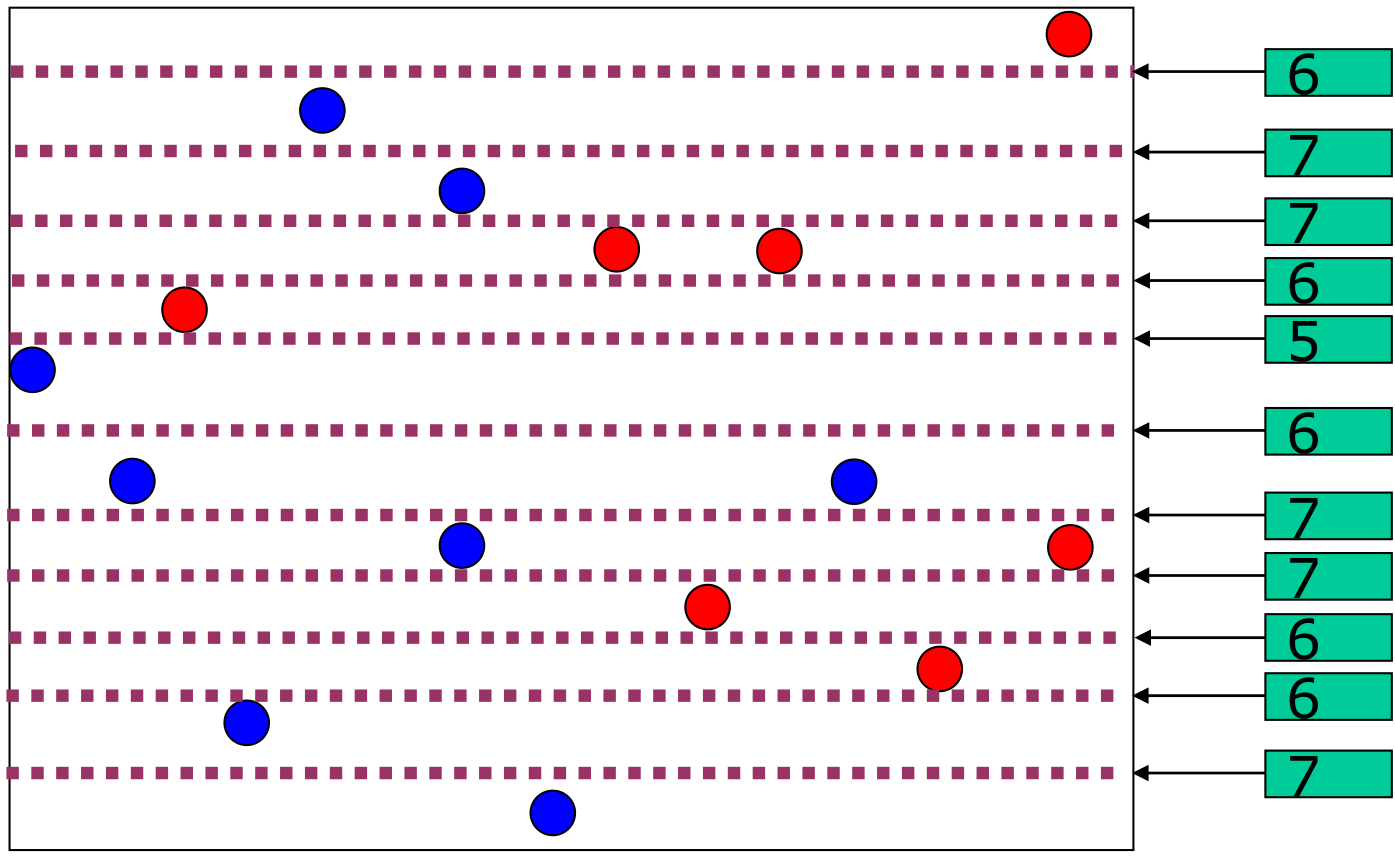
\includegraphics[height=4.5cm,keepaspectratio]{pics/DT-ER-y.png}};
        \node (feat1Txt) [above=1mm of feat1, color=black]  {\emph{y} split AER};
        % \node[inner sep=0pt, visible on=<2>] (feat2) at (0,0)
        %     {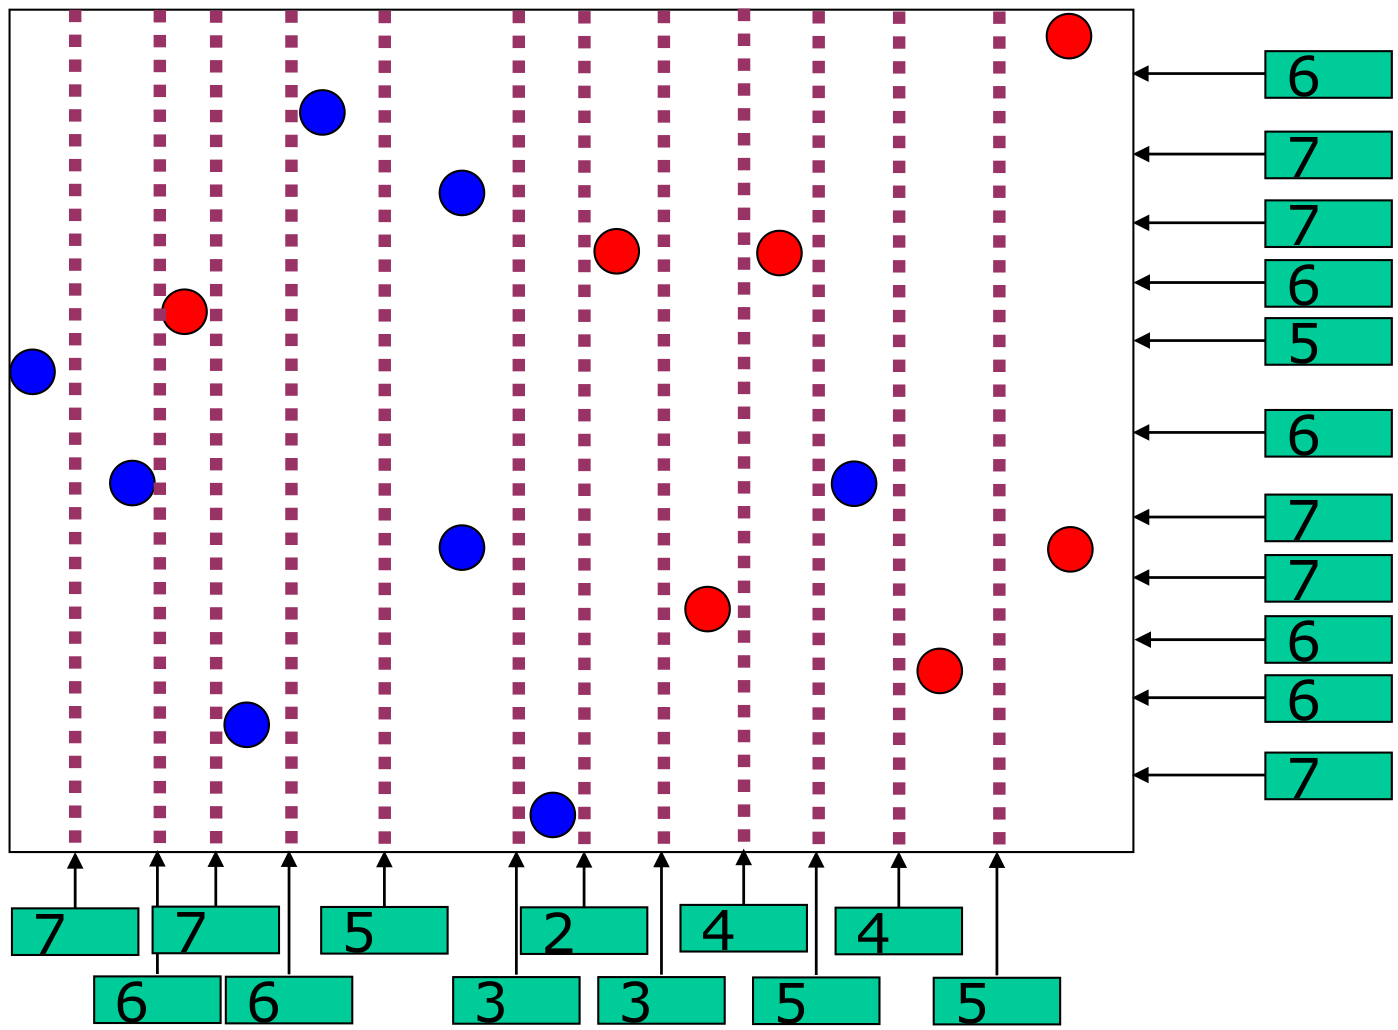
\includegraphics[height=4.5cm,keepaspectratio]{pics/DT-ER-x.png}};
        % \node (feat2Txt) [above=1mm of feat1, color=black,visible on=<2>]  {\emph{x}-\emph{y} split AER};
    \end{tikzpicture}
 
\end{frame}

%------------------------------------------------ 

\begin{frame}
    \frametitle{Decision tree learning}
    1) We compute a measure for \emph{each possible split} in each feature\\\hspace*{5mm}$\to$ here \textbf{absolute error rate} (AER)
    \\
    \vspace*{3mm}
    \centering\begin{tikzpicture}
        \node[inner sep=0pt] (feat2) at (0,0)
            {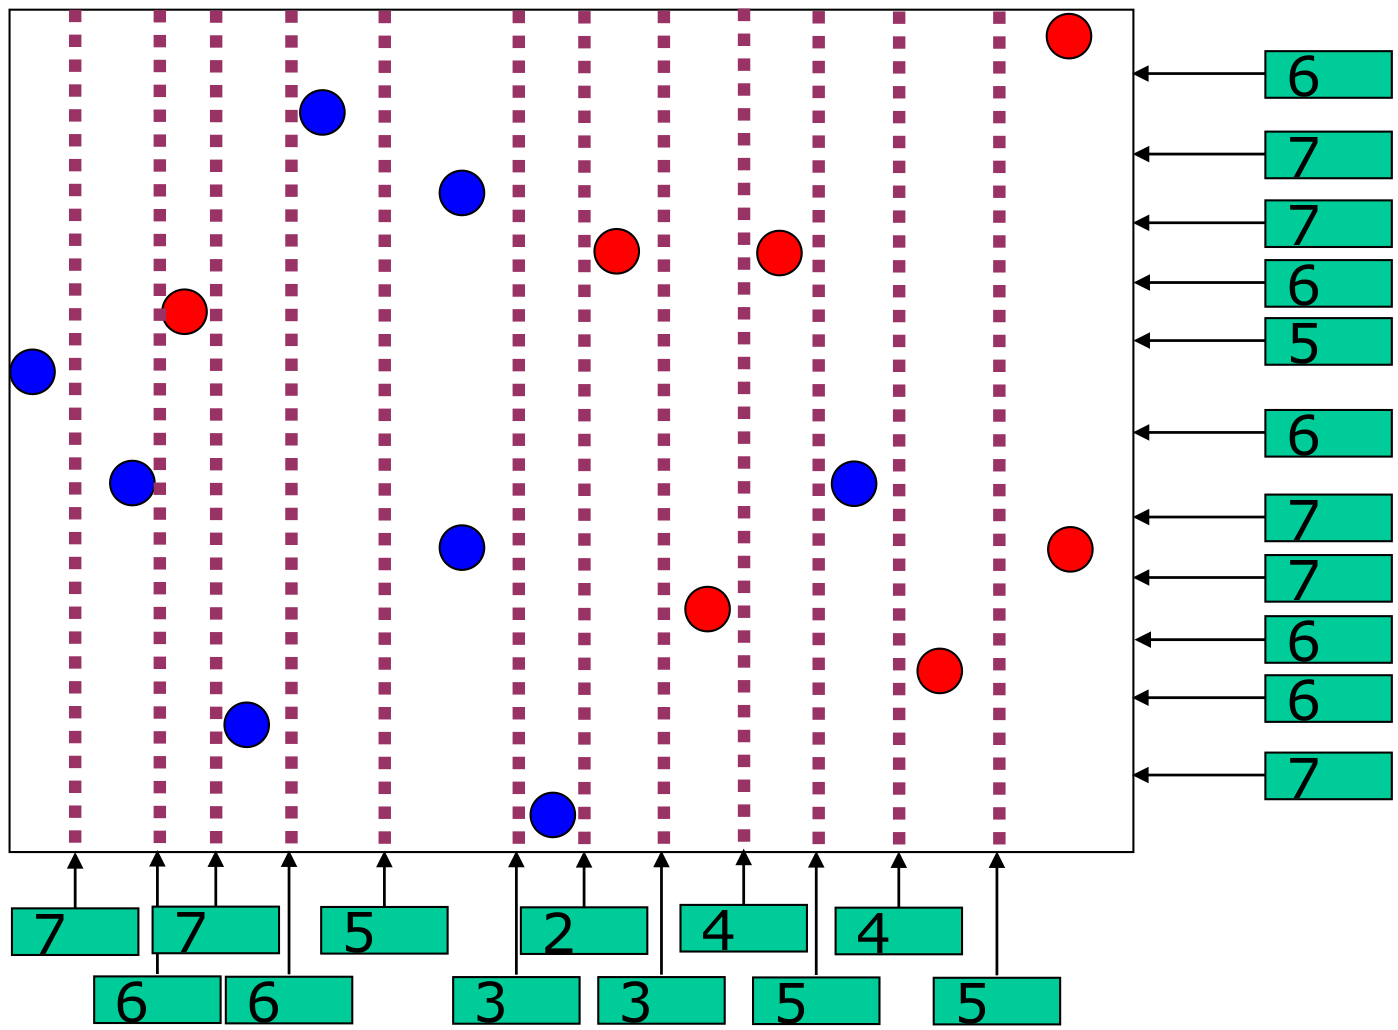
\includegraphics[height=4.5cm,keepaspectratio]{pics/DT-ER-x.png}};
        \node (feat2Txt) [above=1mm of feat1, color=black]  {\emph{x}-\emph{y} split AER};
        \pause
        \node (el) at (-0.53,-1.8) [ellipse, color=red, minimum height=5mm,minimum width=10mm,draw, ultra thick] {};
        \node (txt) at (3.5,-1.8) [color=red, ultra thick] {Minimum AER};
        \draw[->, color=red, ultra thick] (txt) to [out=160, in=20] (el);

    \end{tikzpicture}
 
\end{frame}

%------------------------------------------------ 

\begin{frame}
    \frametitle{Decision tree learning}
    1) We compute a measure for \emph{each possible split} in each feature\\\hspace*{5mm}$\to$ here \textbf{absolute error rate} (AER)\\
    2) Recursively repead step (1) for each subspace until AER $\to 0$
    \\
    \vspace*{3mm}
    \centering\includegraphics<1>[height=4.3cm,keepaspectratio]{pics/DT_1_split.png}%
    \centering\includegraphics<2>[height=4.6cm,keepaspectratio]{pics/DT_2_split.png}%
    \centering\includegraphics<3>[height=4.6cm,keepaspectratio]{pics/DT_3_split.png}%
    \centering\includegraphics<4>[height=4.6cm,keepaspectratio]{pics/DT_4_split.png}%
    \centering\includegraphics<5>[height=4.6cm,keepaspectratio]{pics/DT_5_split.png}%
    \centering\includegraphics<6>[height=4.3cm,keepaspectratio]{pics/DT_final.png}%
     
\end{frame}

%------------------------------------------------ 

\begin{frame}
    \frametitle{Decision tree classification}
    3) Classification
    \\
    \vspace*{3mm}
    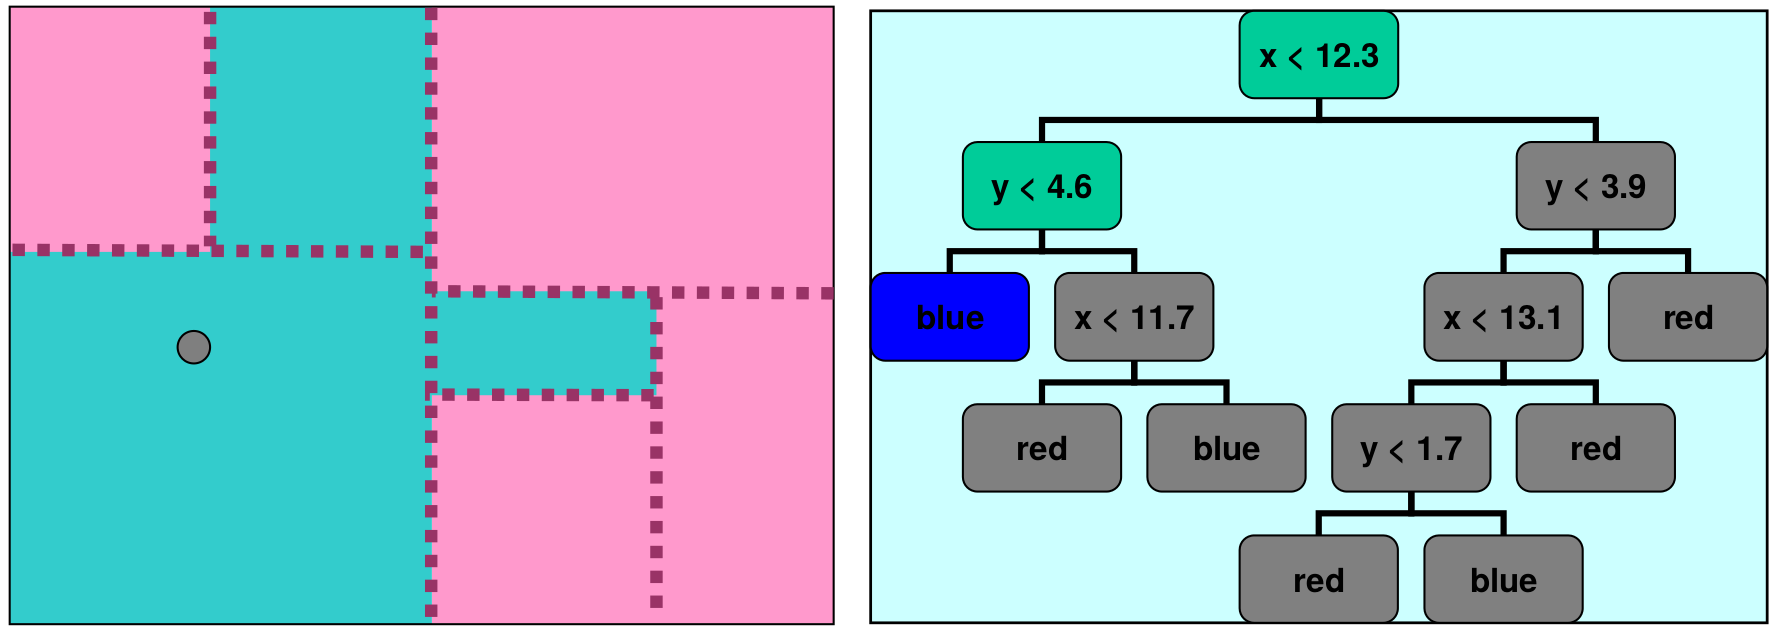
\includegraphics[height=4.3cm,keepaspectratio]{pics/DT_classification.png}%
 
\end{frame}

%------------------------------------------------ 

\begin{frame}
    \frametitle{Decision tree improvements I}
    \begin{itemize}
        \item Use more sophisticated split measures 
            \begin{itemize}
                \item \emph{Information gain} $\leftrightarrow$ (im-)purity of splitted sub-sets
                \item Gini index
            \end{itemize}
        \item Pruning 
    \end{itemize}
    \vspace*{3mm}
    \centering\begin{tikzpicture}
        \node[inner sep=0pt] (IG) at (3,0)
            {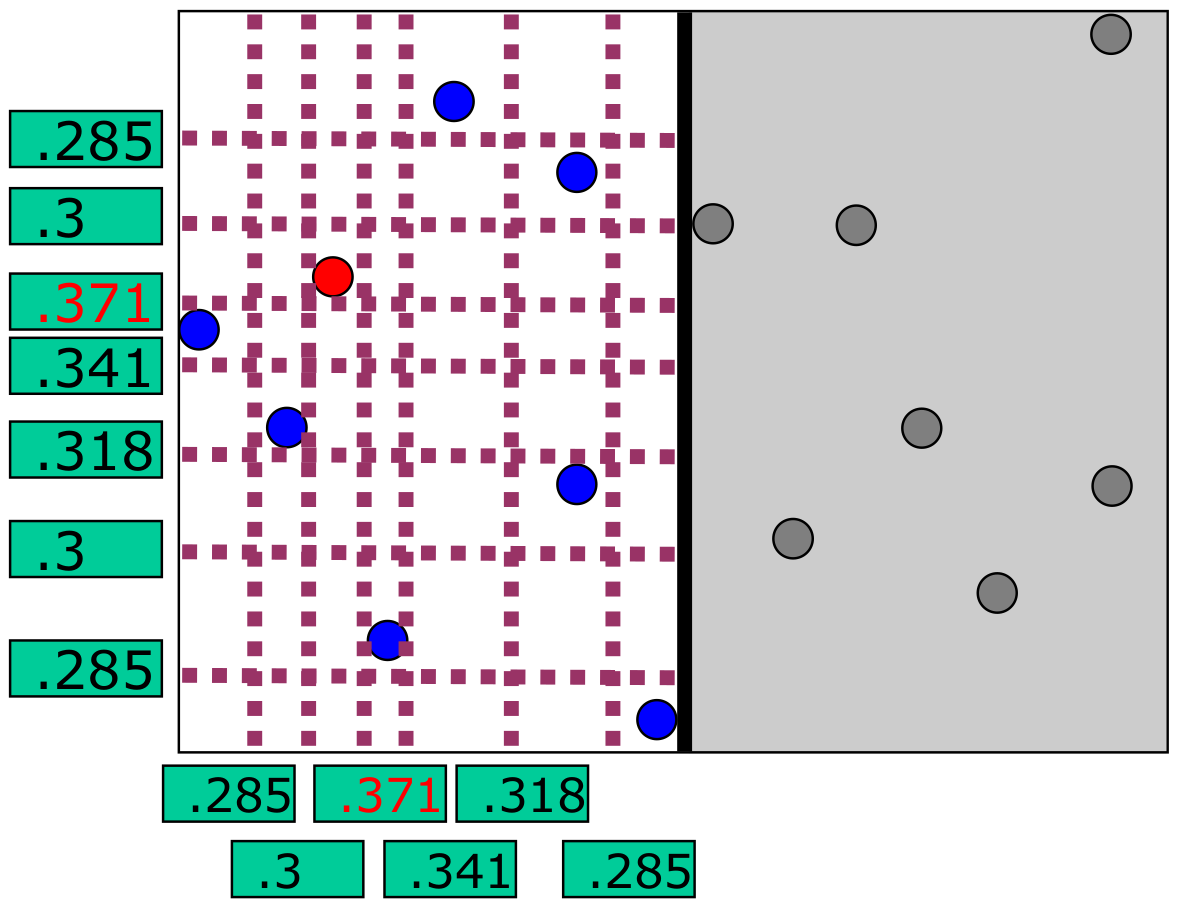
\includegraphics[height=3.5cm,keepaspectratio]{pics/DT_info-gain.png}};
        \node (IGtxt) [below=1mm of IG, color=black]  {Information gain};
        \node[inner sep=0pt] (AER) at (-3,0)
            {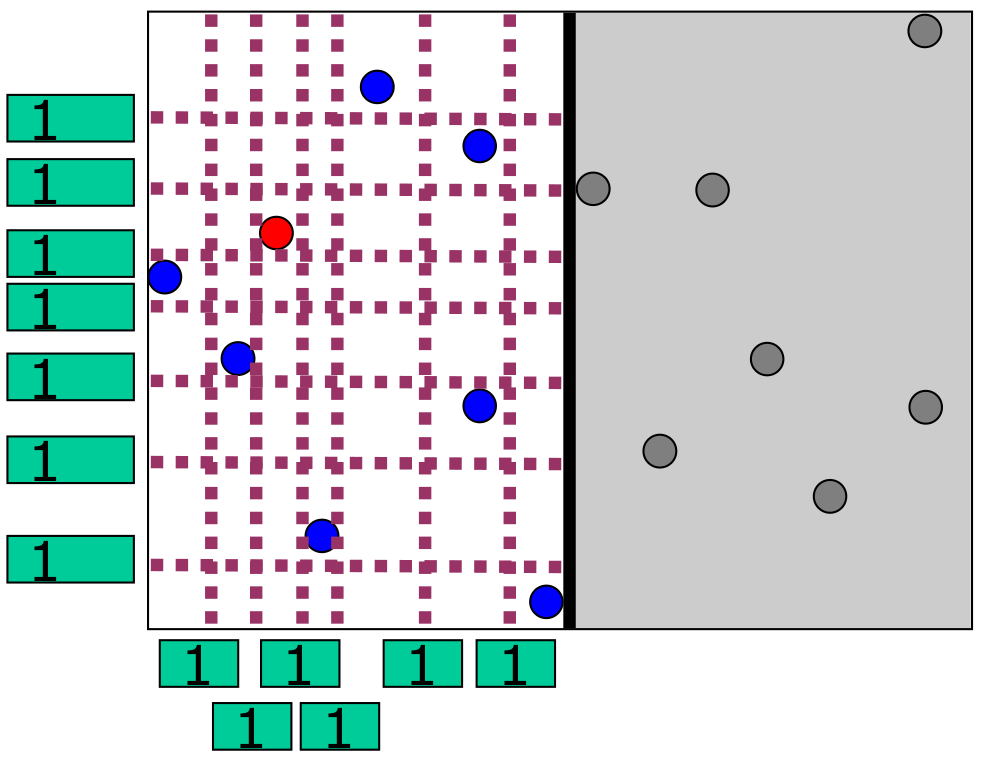
\includegraphics[height=3.5cm,keepaspectratio]{pics/DT_AER.png}};
        \node (AERtxt) [below=1mm of AER, color=black]  {Absolute error rate};
        \draw[->, color=red, ultra thick] (AER) to [out=0, in=180] (IG);
    \end{tikzpicture}
 
\end{frame}

%------------------------------------------------ 

\subsection{Improvements}
\begin{frame}
    \frametitle{Decision tree improvements II}
    \begin{columns}[T] % align columns        
        \begin{column}{.48\textwidth}
            \begin{block}{Random forest}
                \begin{itemize}
                    \item<1-> Ensemble of DTs
                    \item<2-> For each tree use:
                    \begin{itemize}
                        \item<3-> Random sub-sample (=\emph{bootstrapping})
                        \item<4-> Random number of the original features\\
                                  $\to$ large number of rather shallow trees
                    \end{itemize}
                    \item<5-> Classify data by majority voting of individual trees
                \end{itemize}
            \end{block}
        \end{column}%
        \hfill%
        \begin{column}{.48\textwidth}
            \begin{block}{Boosted DT}
                \begin{itemize}
                    \item<6-> Sequential ensemble of evolving DTs
                    \item<7-> Assign weights to training samples $\to$ initially equal weights
                    \item<8-> Adjust weights \& give more importance to misclassified samples
                    \item<9-> Subsequent predictors thus should focus on those 
                \end{itemize}
            \end{block}            
        \end{column}%
    \end{columns}

\end{frame}

%------------------------------------------------ 

\section{Linear cuts}

\begin{frame}
    \frametitle{Linear cuts}
    \begin{columns}[T] % align columns        
        \begin{column}{.48\textwidth}
            % \color{red}\rule{\linewidth}{4pt}
            More degrees of freedom than rectangular cut
            \begin{itemize}
                \item<1-> Simple white box methods 
                \item<2-> Very fast classification
                \item<3-> Can become very powerful by using \emph{kernel trick}
            \end{itemize}
        \end{column}%
        \hfill%
        \begin{column}{.48\textwidth}
            % \color{blue}\rule{\linewidth}{4pt}
            % \hspace*{-10mm}
            \raggedright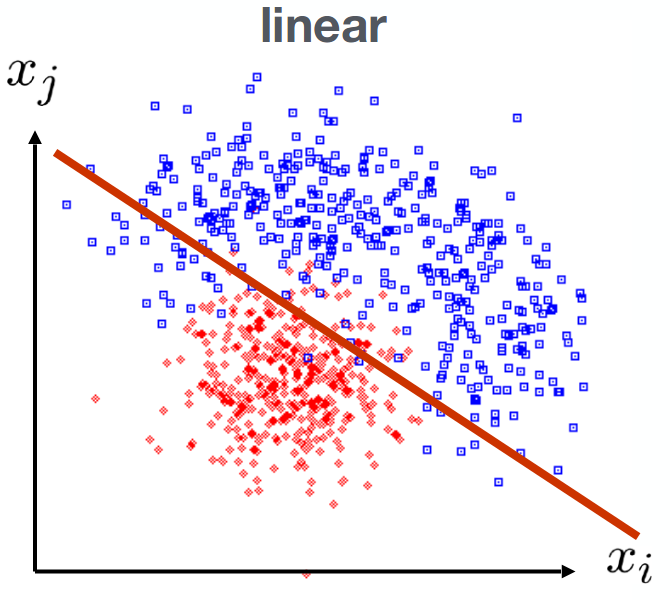
\includegraphics[height=4.3cm,keepaspectratio]{pics/mva_cut_linear.png}%
            
        \end{column}%
    \end{columns}

\end{frame} 

%------------------------------------------------ 

\begin{frame}
    \frametitle{Linear models}
    Takes a \emph{linear function} of its inputs $\boldsymbol{x} = (x_{1},\dots x_{j})$ to base its decision on.\\
    % $$ y = f ( \boldsymbol{w} \cdot \boldsymbol{x}) = f \left\( \sum_{j}w_{j}x_{j} \right\) $$
    $$ y = f (\boldsymbol{w} \cdot \boldsymbol{x}) = f (\sum_{j}w_{j}x_{j}) $$
    
    $\boldsymbol{w}\dots$ weight vector\\ 
    \vspace*{4mm}

    \pause
    Simplest case
    \[ 
         y = f(x)=\Theta(x)=
         \begin{cases} 
             0 & x < 0 \hspace*{5mm}\text{signal}\\
             1  & x \geq 0 \hspace*{5mm}\text{background}
        \end{cases} 
    \] 
    \pause
    \hspace*{5mm}$\to$ Function can be approximated by \textbf{single layer perceptron}
     % Maps all values above certain threshold to \emph{signal} and all others to \emph{background}
    
\end{frame} 

%------------------------------------------------ 
\section{Single layer perceptron}
\begin{frame}
    \frametitle{Single layer perceptron (SLP)}

    \centering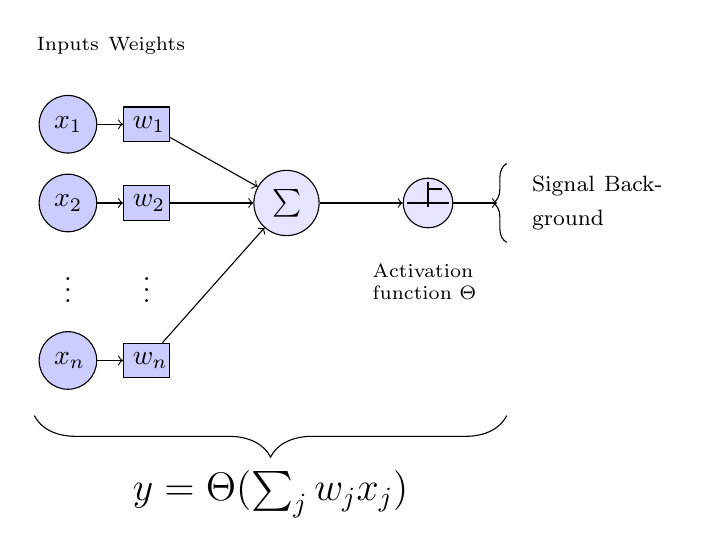
\begin{tikzpicture}
        \node[functions] (center) {};
        \node[below of=center,font=\scriptsize,text width=4em] {Activation function $\Theta$};
        \draw[thick] (0.5em,0.5em) -- (0,0.5em) -- (0,0) -- (-0.5em,0);
        \draw (0em,0.75em) -- (0em,-0.15em);
        \draw (0.75em,0em) -- (-0.75em,0em);
        \node[right of=center] (right) {};
            \path[draw,->] (center) -- (right);
        \node[functions,left=3em of center] (left) {$\sum$};
            \path[draw,->] (left) -- (center);
        \node[weights,left=3em of left] (2) {$w_{2}$} -- (2) node[input,left of=2] (l2) {$x_{2}$};
            \path[draw,->] (l2) -- (2);
            \path[draw,->] (2) -- (left);
        \node[below of=2] (dots) {$\vdots$} -- (dots) node[left of=dots] (ldots) {$\vdots$};
        \node[weights,below of=dots] (n) {$w_{n}$} -- (n) node[input,left of=n] (ln) {$x_{n}$};
            \path[draw,->] (ln) -- (n);
            \path[draw,->] (n) -- (left);
        \node[weights,above of=2] (1) {$w_{1}$} -- (1) node[input,left of=1] (l1) {$x_{1}$};
            \path[draw,->] (l1) -- (1);
            \path[draw,->] (1) -- (left);
        % \node[weights,above of=1] (0) {$w_{0}$} -- (0) node[input,left of=0] (l0) {$1$};
        %     \path[draw,->] (l0) -- (0);
        %     \path[draw,->] (0) -- (left);
        \node[above of=l1,font=\scriptsize] {Inputs};
        \node[above of=1,font=\scriptsize] {Weights};
        \draw [decorate,decoration={brace,mirror,amplitude=15pt},xshift=0pt,yshift=0pt]
            (-5,-2.7) -- (1,-2.7) node [black,midway,yshift=-1.0cm] 
            {\Large $y = \Theta(\sum_{j}w_{j}x_{j})$};
        \draw [decorate,decoration={brace,amplitude=5pt},xshift=0pt,yshift=0pt]
            (1,-0.5) -- (1,0.5) node [text width=5em,black,midway,xshift=1.2cm] 
            {\footnotesize Signal Background};
    \end{tikzpicture}
    
\end{frame} 

%------------------------------------------------ 

\begin{frame}
    \frametitle{SLP training}
    \begin{columns}[T] % align columns        
        \begin{column}{.48\textwidth}
            % \color{red}\rule{\linewidth}{4pt}
            \begin{block}{Algorithm} 
                \begin{enumerate}
                    \item<1-> Initialize weights $\boldsymbol{w}_{init}$
                    \item<2-> Repeat until $y=y_{target}$:
                    \begin{enumerate}
                        \item<3,7,10-> Present training sample $\boldsymbol{x}$
                        \item<4,8,10-> Predict sample label $y=\Theta(\boldsymbol{x}\boldsymbol{w}_{init})$ and compute error $\Delta=y_{target}-y$
                        \item<5,9-> If $\Delta \neq 0~\to$ update weights\\$\boldsymbol{w}\textprime=\boldsymbol{w} + \alpha \Delta \boldsymbol{x}$
                    \end{enumerate}
                \end{enumerate}
            \end{block}
        \end{column}%
        \hfill%
        \begin{column}{.48\textwidth}
            % \color{blue}\rule{\linewidth}{4pt}
            % \hspace*{-10mm}
            \raggedright\includegraphics<1,2>[height=4.3cm,keepaspectratio]{pics/PCT_init_weights.png}%
            \raggedright\includegraphics<3>[height=4.3cm,keepaspectratio]{pics/PCT_0.png}%
            \raggedright\includegraphics<4,5>[height=4.3cm,keepaspectratio]{pics/PCT_1.png}%
            \raggedright\includegraphics<6,7,8>[height=4.3cm,keepaspectratio]{pics/PCT_2.png}%
            \raggedright\includegraphics<9>[height=4.3cm,keepaspectratio]{pics/PCT_3.png}%
            \raggedright\includegraphics<10>[height=4.3cm,keepaspectratio]{pics/PCT_final_0.png}%
            \only<1> {
                \begin{textblock}{3.5}(10,13)
                    $y = w_{1}x_{1} + w_{2}x_{2}$
                \end{textblock}
            }
            \only<5-> {
                \begin{textblock}{5}(2,13)
                    $\alpha \dots$~learning rate
                \end{textblock}
            }
                 
        \end{column}%
    \end{columns}

    

   
\end{frame} 

%------------------------------------------------ 

% next: kernel methods to get non linear DB
% then: MLP how does it get non linear boundary: http://colah.github.io/posts/2014-03-NN-Manifolds-Topology/
%                                                https://cs.stanford.edu/people/karpathy/convnetjs//demo/classify2d.html
%       - show a little how back propergation works -> how weights are adjusted 
%       - state importance that training sample has to represented the unknown samples later on!
% then: measures to quantify MVA performance ROC-AUC etc
% last: show my own analysis



\end{document}

